\titre{OPTRN}
\theme{Réseau de neurones}
\auteur{}
\organisation{AMSCC}
\contenu{
\texte{
Soit le réseau de neurones multicouches décrit pas le graphe suivant:

\begin{center}
	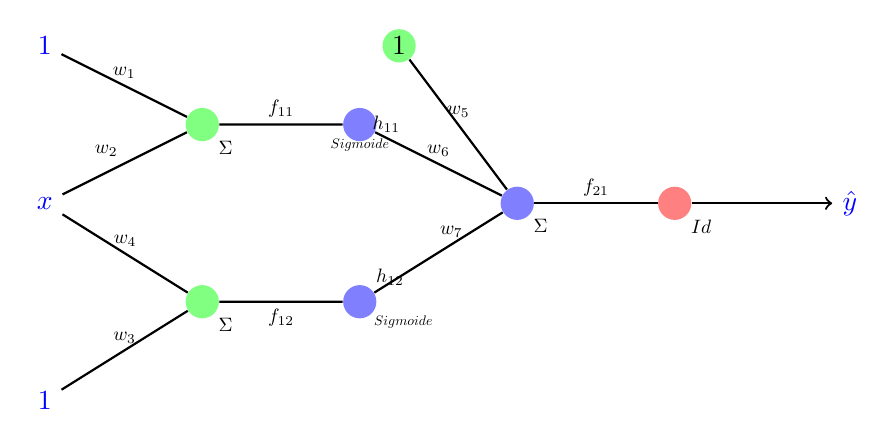
\begin{tikzpicture}[scale=1]
\def\layersep{2cm}
\tikzstyle{every pin edge}=[thick]
\tikzstyle{neuron}=[circle,fill=black!25,minimum size=12pt,inner sep=0pt]
\tikzstyle{entree}=[];
\tikzstyle{input neuron}=[neuron, fill=green!50];
\tikzstyle{output neuron}=[neuron, fill=red!50];
\tikzstyle{hidden neuron}=[neuron, fill=blue!50];
\tikzstyle{annot} = [text width=4em, text centered]

% Entree
\node[entree,blue] (E-1) at (-\layersep,-0.5) {$1$};
\node[entree,blue] (E-2) at (-\layersep,-2.5) {$x$};
\node[entree,blue] (E-3) at (-\layersep,-5) {$1$};

% Premiere couche
%\node[input neuron] (I-1) at (0,-1.25) {};
\node[input neuron] (I-1) at (0,-1.5) {};
\node[input neuron] (I-3) at (0,-3.75) {};

\node[below right=0.8ex,scale=0.7] at (I-1) {$\Sigma$};
%\node[above right=0.8ex,scale=0.7] at (I-2) {$H$};
\node[below right=0.8ex,scale=0.7] at (I-3) {$\Sigma$};

\node[below right=0.8ex,scale=0.7] at (I-1) {};
\node[below right=0.8ex,scale=0.7] at (I-3) {};
%\node[below right=0.8ex,scale=0.7] at (I-2) {};

% \node[above right=0.8ex,blue] at (I-1) {$s_1$};
% \node[above right=0.8ex,blue] at (I-2) {$s_2$};
% \node[above right=0.8ex,blue] at (I-3) {$s_3$};

%Seconde couche et sortie
\node[hidden neuron] (O) at (\layersep,-3.75 cm) {};
\node[hidden neuron] (P) at (\layersep,-1.5 cm) {};
\node[above right=0.8ex,scale=0.7] at (O) {$h_{12}$};
\node[right=0.5ex,scale=0.7] at (P) {$h_{11}$};

% Arrete et poids
\path[thick] (E-1) edge node[pos=0.5,above,scale=0.7]{$w_{1}$} (I-1) ;
\path[thick] (E-2) edge node[pos=0.5,above left,scale=0.7]{$w_{2}$} (I-1);
\path[thick] (E-2) edge node[pos=0.5,above,scale=0.7]{$w_4$} (I-3);
\path[thick] (E-3) edge node[pos=0.5,above,scale=0.7]{$w_3$} (I-3);
\path[thick] (I-1) edge node[pos=0.5,above,scale=0.7]{$f_{11}$} (P);
\path[thick] (I-3) edge node[pos=0.5,below,scale=0.7]{$f_{12}$}(O);
\node[below right=0.8ex,scale=0.5] at (O) {$\text{Sigmoide}$};
\node[below =0.8ex,scale=0.5] at (P) {$\text{Sigmoide}$};
%3eme couche et sortie
\node[hidden neuron] (Q) at (2*\layersep,-2.5 cm) {};
\node[output neuron] (R) at (3*\layersep,-2.5 cm) {};
\node[below right=0.8ex,scale=0.7] at (R) {$\text{Id}$};
\node[input neuron] (I-4) at (2.5,-0.5) {$1$};
\path[thick] (O) edge node[pos=0.6,above,scale=0.7]{$w_{7}$} (Q) ;
\node[below right=0.8ex,scale=0.7] at (Q) {$\Sigma$};
\path[thick] (I-4) edge node[pos=0.5,above,scale=0.7]{$w_{5}$} (Q) ;
\path[thick] (Q) edge node[pos=0.5,above,scale=0.7]{$f_{21}$} (R);
\path[thick] (P) edge node[pos=0.5,above,scale=0.7]{$w_{6}$} (Q) ;
%\path[thick] (E-1) edge node[pos=0.8,above,scale=0.7]{$w_{1}$} (I-1) ;
\draw[->,thick] (R)-- ++(2,0) node[right,blue]{$\hat{y}$};
 %  \node[hidden neuron] (N) at (2*\layersep,-2 cm) {}; % Nouvel neurone de la nouvelle couche
     %           \node[below right=0.8ex,scale=0.7] at (N) {$h_{21}$}; % Nouveau neurone

% Sortie
%\draw[->,thick] (O)-- ++(1,0) node[right,blue]{$F(x,y)$};

\end{tikzpicture}  
\end{center}
\begin{enumerate}
\item Donner les formules qui déterminent les sorties intermédiaires $f_{11},\,f_{12},\,h_{11},\,h_{12}$ et $f_{21}$ ainsi que la sortie finale $\hat{y}$.
\item On pose la fonction d'erreur $E(w)=(y-\hat{y})^2.$ En appliquant l'algorithme de backpropagation, déterminer les dérivées partielles $\frac{\partial E(w)}{\partial w_j}$ puis $\frac{\partial \hat{y}}{\partial w_j}$. En déduire les expressions des mises à jour des paramètres $\Delta w_j$ pour $j=1,\cdots{},7$. 


\end{enumerate}


  }
}
